\documentclass[11pt,a4paper]{article}

\usepackage[margin=1in]{geometry}
\usepackage{fontspec}
\usepackage{graphicx}
\usepackage{xcolor}
\usepackage{booktabs}
\usepackage{tabularx}
\usepackage{array}
\usepackage{float}
\usepackage{caption}
\usepackage{subcaption}
\usepackage{enumitem}
\usepackage{listings}
\usepackage{tikz}
\usepackage{pgfplots}
\usepackage[hidelinks]{hyperref}
\pgfplotsset{compat=1.18}
\usetikzlibrary{arrows.meta, positioning, calc, fit, backgrounds}

\graphicspath{{../../Results/screenshots/}}
% Icon set for the report diagrams.
%
% Same drawing language as the web UI's theme toggle and the ParkingRecog
% icon set (components/Icon.tsx): a 16-unit box, no fill, stroked in the
% current colour, round caps and joins. The moon and sun are copied path for
% path from WebUI/src/theme.js and are the only filled glyphs, as there.
%
% Use inside a tikzpicture:   \pic[scale=1.4] at (x,y) {i-mail};
% Use inline in text:         \icon{i-mail}

\usetikzlibrary{svg.path}

\tikzset{
  icon stroke/.style={line width=0.85pt, line cap=round, line join=round, fill=none},
  % centre the 16x16 box on the pic origin and flip SVG's downward y axis
  icon frame/.style={x=1pt, y=1pt, yscale=-1, shift={(-8,-8)}},
}

\newcommand{\defineicon}[2]{%
  \tikzset{pics/#1/.style={code={%
    \begin{scope}[icon frame]
      \begin{scope}[icon stroke]#2\end{scope}
    \end{scope}}}}}

\newcommand{\icon}[1]{\tikz[baseline=-0.6ex]\pic[scale=0.72]{#1};}

% envelope
\defineicon{i-mail}{
  \draw svg{M3.25 3.75h9.5a1 1 0 0 1 1 1v6.5a1 1 0 0 1-1 1h-9.5a1 1 0 0 1-1-1v-6.5a1 1 0 0 1 1-1z};
  \draw svg{M2.75 4.75 8 8.75l5.25-4};
}
% paper plane: sending
\defineicon{i-send}{
  \draw svg{M13.75 2.25 7.25 8.75};
  \draw svg{M13.75 2.25 9.5 13.75 7.25 8.75 2.25 6.5z};
}
% tray: inbox
\defineicon{i-inbox}{
  \draw svg{M2.25 9h3.25l1 1.75h3l1-1.75h3.25};
  \draw svg{M2.25 9l1.9-5.1a1 1 0 0 1 .95-.65h5.8a1 1 0 0 1 .95.65L13.75 9v3.5a1.25 1.25 0 0 1-1.25 1.25h-9a1.25 1.25 0 0 1-1.25-1.25z};
}
% two stacked units: a mail server
\defineicon{i-server}{
  \draw[rounded corners=1] (2.25,2.25) rectangle (13.75,7);
  \draw[rounded corners=1] (2.25,9) rectangle (13.75,13.75);
  \draw svg{M8 4.6h3.25M8 11.4h3.25};
  \fill (4.75,4.6) circle [radius=.8] (4.75,11.4) circle [radius=.8];
}
% prompt in a window: the CLI
\defineicon{i-terminal}{
  \draw[rounded corners=1.25] (1.75,2.75) rectangle (14.25,13.25);
  \draw svg{M4.5 6.25 6.75 8.25 4.5 10.25M8.5 10.25h3};
}
% window with a title bar: the web UI
\defineicon{i-browser}{
  \draw[rounded corners=1.25] (1.75,2.75) rectangle (14.25,13.25);
  \draw svg{M1.75 5.75h12.5};
  \fill (3.9,4.25) circle [radius=.6] (5.6,4.25) circle [radius=.6];
}
% cylinder: the local mailbox
\defineicon{i-database}{
  \draw (8,4) ellipse [x radius=5.25, y radius=1.75];
  \draw svg{M2.75 4v8c0 .97 2.35 1.75 5.25 1.75s5.25-.78 5.25-1.75V4};
  \draw svg{M2.75 8c0 .97 2.35 1.75 5.25 1.75s5.25-.78 5.25-1.75};
}
% page with a folded corner: a file
\defineicon{i-file}{
  \draw svg{M9.25 1.75H4.25a1 1 0 0 0-1 1v10.5a1 1 0 0 0 1 1h7.5a1 1 0 0 0 1-1V5.25z};
  \draw svg{M9.25 1.75v3.5h3.5};
}
% bulleted lines: the log (ParkingRecog "listview")
\defineicon{i-log}{
  \fill (2.5,4) circle [radius=.8] (2.5,8) circle [radius=.8] (2.5,12) circle [radius=.8];
  \draw svg{M5.75 4h8M5.75 8h8M5.75 12h8};
}
% one figure: the user
\defineicon{i-user}{
  \draw (8,5.5) circle [radius=2.75];
  \draw svg{M2.75 13.75c0-2.6 2.35-4.25 5.25-4.25s5.25 1.65 5.25 4.25};
}
% padlock: authentication
\defineicon{i-lock}{
  \draw[rounded corners=1] (2.75,7.25) rectangle (13.25,13.75);
  \draw (5.25,7.25) -- (5.25,5) arc [start angle=180, end angle=360, radius=2.75] -- (10.75,7.25);
  \draw svg{M8 10v1.25};
}
% clock: timeout
\defineicon{i-clock}{
  \draw (8,8) circle [radius=5.75];
  \draw svg{M8 4.75V8l2.25 1.5};
}
% triangle: warning / error
\defineicon{i-warn}{
  \draw svg{M8 2.25 14.25 13.25H1.75z};
  \draw svg{M8 6.5v3};
  \fill (8,11.4) circle [radius=.75];
}
\defineicon{i-check}{ \draw svg{M3 8.5l3 3 7-7}; }
\defineicon{i-x}{ \draw svg{M4 4l8 8M12 4l-8 8}; }
% plug: TCP connect
\defineicon{i-plug}{
  \draw svg{M5.75 2.25v3M10.25 2.25v3};
  \draw svg{M3.75 5.25h8.5v2.5a4.25 4.25 0 0 1-8.5 0z};
  \draw svg{M8 12v2};
}
% arrow into a tray (ParkingRecog "download"): RETR
\defineicon{i-download}{
  \draw svg{M8 2.25v7.5M5 7.25 8 10.25l3-3M2.5 13.5h11};
}
% sliders (ParkingRecog "setup"): configuration
\defineicon{i-config}{
  \draw svg{M2.25 5.5h2.5M8 5.5h5.75M2.25 10.5h5.5M11.2 10.5h2.55};
  \draw (6.4,5.5) circle [radius=1.6];
  \draw (9.5,10.5) circle [radius=1.6];
}
% ascending bars (ParkingRecog "reports"): performance
\defineicon{i-chart}{
  \draw svg{M2.25 13.75h11.5M5 13.75V9.5M8 13.75V5.5M11 13.75V7.75};
}
% angle brackets: code / the Go core
\defineicon{i-code}{
  \draw svg{M5.5 4.5 2 8l3.5 3.5M10.5 4.5 14 8l-3.5 3.5M9 3 7 13};
}
% the theme toggle's two glyphs, exactly as drawn in WebUI/src/theme.js
\tikzset{pics/i-moon/.style={code={\begin{scope}[icon frame]
  \fill svg{M13.3 9.9A5.9 5.9 0 0 1 6.1 2.7a5.9 5.9 0 1 0 7.2 7.2z};
\end{scope}}}}
\tikzset{pics/i-sun/.style={code={\begin{scope}[icon frame]
  \fill (8,8) circle [radius=3.1];
  \draw[icon stroke, line width=1.1pt] svg{M8 1.1v1.7M8 13.2v1.7M1.1 8h1.7M13.2 8h1.7M3.2 3.2l1.2 1.2M11.6 11.6l1.2 1.2M12.8 3.2l-1.2 1.2M4.4 11.6l-1.2 1.2};
\end{scope}}}}


% Basic information
\newcommand{\coursename}{Computer Network Course Practice}
\newcommand{\projecttitle}{Design and Implementation of a Lightweight Email Client}
\newcommand{\semester}{2026 Fall}
\newcommand{\schoolname}{School of Computer Science and Technology}
\newcommand{\universityname}{Beijing Institute of Technology}

% Replace these before submission.
\newcommand{\studentid}{1820232064}{\rule{7cm}{0.4pt}}
\newcommand{\studentname}{杨辉宗}{\rule{7cm}{0.4pt}}
\newcommand{\reportdate}{2026年10月11日}{\rule{7cm}{0.4pt}}

% Simple instruction text used throughout the template.
\newcommand{\prompt}[1]{\textit{#1}}

% ---- report styling -------------------------------------------------------
\definecolor{accent}{RGB}{37,99,235}     % client side, commands
\definecolor{reply}{RGB}{71,85,105}      % server side, replies
\definecolor{okc}{RGB}{21,128,61}
\definecolor{errc}{RGB}{185,28,28}
\definecolor{panel}{RGB}{246,247,250}
\definecolor{rule}{RGB}{203,213,225}

\setlength{\parskip}{0.45em}
\setlength{\parindent}{0pt}
\captionsetup{font=small, labelfont=bf}
\setlist{itemsep=0.15em, topsep=0.3em}
\renewcommand{\arraystretch}{1.18}

\lstdefinelanguage{Go}{
  morekeywords={func,return,if,else,for,range,var,type,struct,defer,package,import,nil,err,switch,case,default,go,chan,map,interface,const},
  sensitive=true, morecomment=[l]{//}, morestring=[b]",
}
\lstset{
  basicstyle=\ttfamily\footnotesize, columns=fullflexible, keepspaces=true,
  frame=single, rulecolor=\color{rule}, backgroundcolor=\color{panel},
  framesep=4pt, xleftmargin=4pt, xrightmargin=4pt,
  keywordstyle=\color{accent}\bfseries, commentstyle=\color{reply}\itshape,
  stringstyle=\color{okc}, showstringspaces=false, breaklines=true,
}
\lstdefinestyle{wire}{language={}, keywordstyle={}, stringstyle={}}

% diagram styles
\tikzset{
  >=Stealth,
  box/.style={draw=rule, fill=panel, rounded corners=3pt, line width=0.6pt,
              inner sep=5pt, align=center, font=\small},
  cbox/.style={box, draw=accent!60, fill=accent!6},
  sbox/.style={box, draw=reply!50, fill=reply!6},
  lbl/.style={font=\scriptsize\ttfamily, inner sep=1.5pt},
  note/.style={font=\scriptsize, text=reply, align=left},
  flow/.style={->, line width=0.8pt, draw=reply},
  cmd/.style={->, line width=0.8pt, draw=accent},
  rep/.style={->, line width=0.8pt, draw=reply, dashed},
  life/.style={draw=rule, line width=1pt},
}

\begin{document}

% -------------------------------------------------
% Cover page
% -------------------------------------------------
\begin{titlepage}
\centering

\vspace*{2cm}

{\Large \coursename\par}

\vspace{2cm}

{\LARGE\bfseries \projecttitle\par}

\vspace{0.8cm}

{\Large Report\par}

\vfill

\begin{tabular}{ll}
Student ID: & \studentid \\[1em]
Name:       & \studentname \\[1em]
Date:       & \reportdate
\end{tabular}

\vfill

{\schoolname\par}
{\universityname\par}

\vspace{0.8cm}

{\semester\par}

\end{titlepage}

\tableofcontents
\newpage

% =================================================
\section{Requirements}
% =================================================

The project is a lightweight email client that talks to mail servers over plain TCP
sockets. It supports one account on one test server, sends plain-text mail with a subset
of SMTP, receives mail with a subset of POP3, shows an Inbox, and keeps downloaded
messages in a local file so they are still there after a restart. The protocol code is
written directly against the socket; no library that hides SMTP or POP3 is used.

\subsection{Basic requirements and what was implemented}

Table~\ref{tab:req} lists every required function from the project description (§2) and
where it is implemented. All of them are complete.

\begin{table}[H]
\centering\small
\caption{Required functions (project description §2) and their implementation.}
\label{tab:req}
\begin{tabularx}{\linewidth}{@{} l X l c @{}}
\toprule
& \textbf{Requirement} & \textbf{Where} & \\
\midrule
\icon{i-config} & One account and one test server; address, SMTP port, POP3 port, username and
  other settings in a configuration file; clear errors when the server is unreachable or
  login fails & \texttt{config.json}, \texttt{pkg/config} & \textcolor{okc}{\icon{i-check}} \\
\icon{i-send} & Send plain text to one or more recipients with \texttt{EHLO}/\texttt{HELO},
  \texttt{MAIL FROM}, \texttt{RCPT TO}, \texttt{DATA}, \texttt{QUIT}; user enters
  recipients, subject and body & \texttt{pkg/smtp} & \textcolor{okc}{\icon{i-check}} \\
\icon{i-inbox} & Receive with \texttt{USER}/\texttt{PASS}, \texttt{STAT}/\texttt{LIST},
  \texttt{RETR}, \texttt{QUIT}; Inbox shows number, sender, subject, date; user selects
  and reads one message & \texttt{pkg/pop3}, \texttt{pkg/message} & \textcolor{okc}{\icon{i-check}} \\
\icon{i-database} & Save downloaded messages locally and view them again after a restart
  & \texttt{pkg/mailbox} (JSON) & \textcolor{okc}{\icon{i-check}} \\
\icon{i-terminal} & User interface: the five-item menu (Check Inbox, Read Message, Compose
  and Send, View Local Messages, Exit) & \texttt{cmd/cli} & \textcolor{okc}{\icon{i-check}} \\
\icon{i-warn} & Survive connection failure, timeout, wrong password, unexpected
  response, interrupted transfer and invalid input without crashing
  & \texttt{pkg/mailerr} & \textcolor{okc}{\icon{i-check}} \\
\icon{i-log} & Log important events; never write a password to the log
  & \texttt{pkg/logger}, \texttt{pkg/pop3} & \textcolor{okc}{\icon{i-check}} \\
\bottomrule
\end{tabularx}
\end{table}

\subsection{Bonus features}

These go beyond the basic requirements and are kept separate from them. The command-line
client does not depend on any of them.

\begin{itemize}
  \item \icon{i-browser} \textbf{Graphical interface} (listed bonus). A web interface built with
        Vite and Tailwind CSS. It talks to a small JSON API in the Go program
        (\texttt{cmd/serve}), which uses exactly the same SMTP, POP3 and mailbox code as the CLI.
        It has Inbox, Read, Compose and Saved screens, a live SMTP/POP3 status light, and works
        at phone width.
  \item \icon{i-user} \textbf{Multiple accounts} (listed bonus). In the web interface any account
        on the mail server can sign in. The password is checked with a real POP3
        \texttt{USER}/\texttt{PASS} exchange, and each account gets its own saved mailbox
        under \texttt{data/accounts/<email>/}.
  \item \icon{i-code} \textbf{Safe concurrency} (part of the ``improved concurrency'' bonus). The HTTP
        server handles each request on its own goroutine. The mailbox is guarded by a
        read/write lock, and POP3 sessions for one account are serialised by a mutex, while
        sending is not blocked by a running download. The whole test suite passes under
        Go's race detector.
  \item \textbf{Small extras}: a profile picture per account, and a light/dark theme toggle
        (\icon{i-sun}\,/\,\icon{i-moon}) carried over from an earlier project of mine.
\end{itemize}

Not implemented: TLS/STARTTLS, MIME attachments, IMAP, HTML mail, background checking.

% =================================================
\section{Analysis}
% =================================================

\subsection{SMTP: a command--reply protocol with numeric codes}

SMTP (RFC 5321~\cite{rfc5321}) is a text protocol on TCP. The client sends one command per
line, ended with \verb|\r\n|, and the server answers each command with a reply whose
first three characters are a status code. The first digit carries the meaning:
\texttt{2xx} success, \texttt{3xx} ``go on, send more'' (only \texttt{354} after
\texttt{DATA}), \texttt{4xx} temporary failure, \texttt{5xx} permanent failure. The client
therefore must check each code before it sends the next command; for example, it must not
send the message body unless \texttt{DATA} was answered with \texttt{354}.

The codes this client expects are: \texttt{220} greeting, \texttt{250} for
\texttt{EHLO}, \texttt{MAIL FROM}, \texttt{RCPT TO} and the end of data, \texttt{354} for
\texttt{DATA}, and \texttt{221} for \texttt{QUIT}. Two details of the reply format matter:

\begin{itemize}
  \item \textbf{Multi-line replies.} A reply can span several lines. \texttt{250-text} (code,
        hyphen) means more lines follow; \texttt{250 text} (code, space) is the last line.
        GreenMail answers \texttt{EHLO} with three lines, so reading ``one line'' would
        leave two lines unread and every later reply would be matched to the wrong command.
  \item \textbf{End of data and dot-stuffing.} After \texttt{354} the message is sent as
        lines and ended by a line holding only a dot (\verb|\r\n.\r\n|). A body line that
        itself starts with a dot must be sent with an extra dot (``\texttt{..}''), and the
        receiver removes it again. Without this a body line containing just ``\texttt{.}''
        would end the message early.
\end{itemize}

\subsection{POP3: status lines and dot-terminated lists}

POP3 (RFC 1939~\cite{rfc1939}) has no numeric codes. Every reply starts with
\texttt{+OK} or \texttt{-ERR}. Replies to \texttt{LIST} and \texttt{RETR} are multi-line:
after the \texttt{+OK} line the server sends data lines and ends them with a single dot,
with the same dot-stuffing rule as SMTP. A session goes through three states:
\emph{authorization} (\texttt{USER}, \texttt{PASS}), \emph{transaction} (\texttt{STAT},
\texttt{LIST}, \texttt{RETR}) and \emph{update}, which begins at \texttt{QUIT}. Two
consequences shaped the design:

\begin{itemize}
  \item Message numbers are only valid inside one session. Message 1 today may be another
        message tomorrow. So the local mailbox gives every saved message its own permanent
        ID instead of reusing the POP3 number.
  \item The server locks the maildrop while a session is open, so a second parallel login
        for the same account is refused. The client must not run two POP3 sessions for one
        account at the same time.
\end{itemize}

\subsection{TCP is a byte stream}

TCP delivers an ordered stream of bytes, not messages. One \texttt{write} by the server can
arrive in several \texttt{read} calls, and one \texttt{read} can contain the end of one reply
and the start of the next. This was measured in this project: a raw socket received a
104\,KB \texttt{RETR} reply from GreenMail in \textbf{672 separate reads}, about 155 bytes
each (Section~\ref{sec:perf}). The protocol layer therefore must buffer the incoming bytes
and cut them into lines at \verb|\r\n|, and then decide from the line content whether a reply
is finished: by the space after the code in SMTP, or by the lone dot in POP3 multi-line
replies. Figure~\ref{fig:stream} shows this in the client.

\subsection{Message format}

The text after \texttt{DATA} and the text returned by \texttt{RETR} follow the Internet
Message Format (RFC 5322~\cite{rfc5322}): header lines such as \texttt{From:},
\texttt{To:}, \texttt{Subject:} and \texttt{Date:}, a blank line, then the body. For the
Inbox the client needs sender, subject and date, which it reads from these headers. A
subject with non-ASCII characters is written as an RFC 2047 encoded word~\cite{rfc2047},
e.g.\ \texttt{=?utf-8?q?caf=C3=A9?=}, and has to be decoded for display.

\subsection{Local storage}

The spec allows text files, JSON or SQLite. A single JSON file was chosen: it needs no
extra software, can be opened and checked by hand, and is fast enough for a personal
mailbox of a few hundred messages. Two problems had to be handled: pressing ``Check Inbox''
twice must not save every message twice, and a crash while saving must not destroy the file.

\subsection{Failure cases}

Each failure appears at a different layer and must be told apart so the user gets a useful
message:

\begin{table}[H]
\centering\small
\begin{tabularx}{\linewidth}{@{} l l X @{}}
\toprule
& \textbf{Failure} & \textbf{How it shows up} \\
\midrule
\icon{i-plug} & Server unreachable & \texttt{connect} fails with ``connection refused'', or a DNS error \\
\icon{i-clock} & Timeout & a socket read or write passes its deadline \\
\icon{i-lock} & Wrong username/password & POP3 answers \texttt{USER} or \texttt{PASS} with \texttt{-ERR} \\
\icon{i-x} & Server refuses & SMTP \texttt{4xx}/\texttt{5xx} (e.g.\ \texttt{550} on \texttt{RCPT}), or another POP3 \texttt{-ERR} \\
\icon{i-warn} & Unexpected response & a line that is not \texttt{NNN text} or \texttt{+OK}/\texttt{-ERR} \\
\icon{i-download} & Interrupted transfer & the socket closes before the terminating dot (EOF, reset) \\
\icon{i-terminal} & Invalid input & bad menu choice, non-numeric message number, malformed address \\
\bottomrule
\end{tabularx}
\end{table}

\subsection{Choice of test server}

The client was developed against \textbf{GreenMail}~\cite{greenmail}, an open-source test
mail server that provides SMTP and POP3 in one Docker container. It was chosen because it is
an independent, standard implementation, so the client is tested against a server I did not
write; it checks passwords, which the wrong-password test needs; it runs on
\texttt{localhost} with no TLS or OAuth, which the basic project leaves out; and it is
started and reset with one command, which makes the tests repeatable. It listens on ports
3025 (SMTP) and 3110 (POP3) instead of 25 and 110, which need administrator rights.

% =================================================
\section{Design}
% =================================================

\subsection{Architecture}

The client is split into small Go packages with one job each (Figure~\ref{fig:arch}). Two
thin front ends, the CLI and the HTTP API for the web interface, sit on one shared core.
The protocol code exists exactly once, so both front ends send and receive mail in the same
way and the tests of the core cover both.

\begin{figure}[H]
\centering
\begin{tikzpicture}[node distance=6mm and 6mm]
  % front ends
  \node[cbox, minimum width=3.3cm, minimum height=1.25cm] (cli) at (0,0) {\\[1.05em]\textbf{CLI}\\[-1pt]\scriptsize\texttt{cmd/cli}};
  \pic[scale=1.25, accent] at ($(cli.north)+(0,-0.33)$) {i-terminal};
  \node[cbox, minimum width=3.3cm, minimum height=1.25cm] (api) at (5.2,0) {\\[1.05em]\textbf{HTTP API}\\[-1pt]\scriptsize\texttt{cmd/serve}, \texttt{pkg/server}};
  \pic[scale=1.25, accent] at ($(api.north)+(0,-0.33)$) {i-code};
  \node[cbox, minimum width=2.6cm, minimum height=1.25cm] (web) at (9.8,0) {\\[1.05em]\textbf{Web UI}\\[-1pt]\scriptsize Vite + Tailwind};
  \pic[scale=1.25, accent] at ($(web.north)+(0,-0.33)$) {i-browser};
  \node[cbox, minimum width=1.4cm, minimum height=1.25cm] (usr) at (-3.0,0) {\\[1.05em]\textbf{User}};
  \pic[scale=1.25, accent] at ($(usr.north)+(0,-0.33)$) {i-user};

  \draw[flow] (usr) -- node[above, lbl]{menu} (cli);
  \draw[flow, <->] (web) -- node[above, lbl]{JSON} (api);

  % core
  \node[box, minimum width=8.5cm, minimum height=0.9cm] (acct) at (2.6,-1.9)
     {\textbf{account} \quad\scriptsize Send $\cdot$ Refresh $\cdot$ Fetch $\cdot$ Local \quad (one POP3 session at a time)};
  \draw[flow] (cli) -- (cli |- acct.north);
  \draw[flow] (api) -- (api |- acct.north);

  % packages
  \foreach \n/\x/\ic/\t/\s in {smtp/-1.2/i-send/smtp/RFC 5321, pop3/1.35/i-inbox/pop3/RFC 1939, msg/3.9/i-mail/message/RFC 5322, mb/6.45/i-database/mailbox/JSON file}{
    \node[box, minimum width=2.25cm, minimum height=1.35cm] (\n) at (\x,-3.75) {\\[1.05em]\textbf{\t}\\[-1pt]\scriptsize\s};
    \pic[scale=1.25] at ($(\n.north)+(0,-0.35)$) {\ic};
    \draw[flow] (\x,-2.35) -- (\n.north);
  }
  % cross-cutting
  \node[box, minimum width=1.9cm, minimum height=0.95cm, anchor=west] (lg) at (8.3,-1.6) {\textbf{logger}\\[-1pt]\scriptsize slog, redaction};
  \node[box, minimum width=1.9cm, minimum height=0.95cm, anchor=west] (me) at (8.3,-2.75) {\textbf{mailerr}\\[-1pt]\scriptsize error kinds};
  \node[box, minimum width=1.9cm, minimum height=0.95cm, anchor=west] (cf) at (8.3,-3.9) {\textbf{config}\\[-1pt]\scriptsize \texttt{config.json}};

  % outside world
  \node[sbox, minimum width=4.9cm, minimum height=1.35cm] (gm) at (0.075,-6.1) {\\[1.05em]\textbf{GreenMail} \scriptsize SMTP :3025 $\cdot$ POP3 :3110};
  \pic[scale=1.25, reply] at ($(gm.north)+(0,-0.35)$) {i-server};
  \node[sbox, minimum width=2.25cm, minimum height=1.35cm] (file) at (6.45,-6.1) {\\[1.05em]\scriptsize\texttt{data/mailbox.json}};
  \pic[scale=1.25, reply] at ($(file.north)+(0,-0.35)$) {i-file};
  \node[sbox, minimum width=1.9cm, minimum height=1.35cm, anchor=west] (logf) at (8.3,-6.1) {\\[1.05em]\scriptsize\texttt{logs/client.log}};
  \pic[scale=1.25, reply] at ($(logf.north)+(0,-0.35)$) {i-log};

  \draw[flow, <->] (smtp.south) -- node[left, lbl]{TCP} (smtp.south |- gm.north);
  \draw[flow, <->] (pop3.south) -- node[right, lbl]{TCP} (pop3.south |- gm.north);
  \draw[flow, <->] (mb) -- (file);
  \draw[flow] (lg.east) -- ++(0.35,0) |- (logf.east);
  \draw[flow, dotted] (msg) -- (pop3);
  \draw[flow, dotted] (msg) -- (mb);
\end{tikzpicture}
\caption{Module structure. Blue: front ends. Grey: the shared core and the outside world.
         \texttt{logger}, \texttt{mailerr} and \texttt{config} are used by every package. Only \texttt{smtp} and \texttt{pop3} open sockets; \texttt{message} only builds and
         parses text.}
\label{fig:arch}
\end{figure}

\begin{table}[H]
\centering\small
\caption{Module responsibilities.}
\begin{tabularx}{\linewidth}{@{} l X @{}}
\toprule
\textbf{Package} & \textbf{Responsibility} \\
\midrule
\texttt{config}  & Load \texttt{config.json}, apply defaults, reject unknown keys, report \emph{all} invalid fields at once. The password may come from \texttt{EMAIL\_PASSWORD} instead of the file. \\
\texttt{logger}  & Structured log (\texttt{log/slog}) to \texttt{logs/client.log}; any attribute named \texttt{password}, \texttt{pass} or \texttt{secret} is replaced by \texttt{[REDACTED]}. \\
\texttt{smtp}    & One SMTP session over a raw socket: greeting, \texttt{EHLO} (fallback \texttt{HELO}), \texttt{MAIL FROM}, \texttt{RCPT TO} per recipient, \texttt{DATA}, \texttt{QUIT}. Checks every reply code. \\
\texttt{pop3}    & POP3 over a raw socket: \texttt{USER}/\texttt{PASS}, \texttt{STAT}, \texttt{LIST}, \texttt{RETR}, \texttt{QUIT}. Parses \texttt{+OK}/\texttt{-ERR}; masks \texttt{PASS} in the log. \\
\texttt{message} & Build the outgoing text (headers + body); parse incoming text into From, To, Subject, Date, Body; validate recipient addresses. \\
\texttt{mailbox} & Local store: add with duplicate check (SHA-256), permanent local IDs, atomic save to JSON. \\
\texttt{account} & The four use cases (send, refresh inbox, fetch one, list local) shared by both front ends. \\
\texttt{mailerr} & Turn any error into one of eight kinds and a plain-language sentence. \\
\texttt{server}  & HTTP JSON handlers, sign-in sessions, static files for the web UI. \\
\bottomrule
\end{tabularx}
\end{table}

\subsection{Main data flow: sending and receiving}

Figure~\ref{fig:flow} follows one message through the whole system. On the way out the
client builds the message text and hands it to the SMTP session. GreenMail stores it in the
recipient's maildrop. On the way in a POP3 session lists and retrieves it, the text is parsed
into fields, and the mailbox saves it with a new local ID. The Inbox is drawn from that saved
copy.

\begin{figure}[H]
\centering
\begin{tikzpicture}[x=1cm, y=1cm]
  \tikzset{st/.style={box, minimum width=2.2cm, minimum height=1.55cm, text width=2.0cm}}
  \newcommand{\step}[6]{%
    \node[#5, st] (#1) at (#2) {\\[1.0em]\textbf{#3}\\[-1pt]\scriptsize #4};
    \pic[scale=1.35, #6] at ($(#1.north)+(0,-0.38)$) {#1};}
  % send row
  \node[font=\small\bfseries, text=accent, anchor=west] at (-1.2,1.35) {Send};
  \step{i-user}{0,0}{Compose}{to, subject, body}{cbox}{accent}
  \step{i-mail}{2.75,0}{Build}{headers + body\\ \texttt{message.Build}}{cbox}{accent}
  \step{i-send}{5.5,0}{SMTP}{EHLO $\rightarrow$ QUIT\\ \texttt{smtp.Send}}{cbox}{accent}
  \step{i-server}{9.6,-1.6}{GreenMail}{stores in the recipient's maildrop}{sbox}{reply}
  % receive row
  \node[font=\small\bfseries, text=okc, anchor=west] at (-1.2,-1.85) {Receive};
  \node[box, st, draw=okc!60, fill=okc!5] (i-inbox) at (5.5,-3.2) {\\[1.0em]\textbf{POP3}\\[-1pt]\scriptsize LIST, RETR\\ \texttt{Refresh}};
  \pic[scale=1.35, okc] at ($(i-inbox.north)+(0,-0.38)$) {i-inbox};
  \node[box, st, draw=okc!60, fill=okc!5] (i-code) at (2.75,-3.2) {\\[1.0em]\textbf{Parse}\\[-1pt]\scriptsize From, Subject, Date\\ \texttt{message.Parse}};
  \pic[scale=1.35, okc] at ($(i-code.north)+(0,-0.38)$) {i-code};
  \node[box, st, draw=okc!60, fill=okc!5] (i-database) at (0,-3.2) {\\[1.0em]\textbf{Save}\\[-1pt]\scriptsize dedupe, local ID\\ \texttt{mailbox.json}};
  \pic[scale=1.35, okc] at ($(i-database.north)+(0,-0.38)$) {i-database};
  \node[box, st, draw=okc!60, fill=okc!5] (i-terminal) at (-2.75,-3.2) {\\[1.0em]\textbf{Show}\\[-1pt]\scriptsize Inbox table,\\ read message};
  \pic[scale=1.35, okc] at ($(i-terminal.north)+(0,-0.38)$) {i-terminal};

  \draw[flow, draw=accent] (i-user) -- (i-mail);
  \draw[flow, draw=accent] (i-mail) -- (i-send);
  \draw[flow, draw=accent] (i-send.east) -| node[pos=0.25, above, lbl]{TCP :3025} (i-server.north);
  \draw[flow, draw=okc] (i-server.south) |- node[pos=0.75, below, lbl]{TCP :3110} (i-inbox.east);
  \draw[flow, draw=okc] (i-inbox) -- (i-code);
  \draw[flow, draw=okc] (i-code) -- (i-database);
  \draw[flow, draw=okc] (i-database) -- (i-terminal);
  \draw[flow, dashed, draw=okc] (i-database.south) -- ++(0,-0.55) node[below, note]{after a restart: View Local Messages reads the file, no network};
\end{tikzpicture}
\caption{The path of one message from Compose to the Inbox.}
\label{fig:flow}
\end{figure}

\subsection{Design decisions}

\begin{itemize}
  \item \textbf{One session per action.} Every send and every inbox check opens a new
        connection and closes it with \texttt{QUIT}. There is no long-lived connection to
        keep alive or to recover after a network error.
  \item \textbf{A fresh deadline before every step.} The socket deadline is reset before each
        command, so a slow but working server is fine while a server that stops answering
        fails after \texttt{timeout\_seconds} instead of hanging forever.
  \item \textbf{Local ID separate from POP3 number.} The Inbox and ``Read Message'' use the
        server's number for the current session; the saved copy keeps a local ID that never
        changes and is never reused.
  \item \textbf{Errors are values, handled in one place.} Every function returns an error
        wrapped with the step that failed (e.g.\ \texttt{smtp: RCPT TO bob@x: 550 ...}). The
        CLI menu loop and the HTTP handler each pass it to \texttt{mailerr.Explain} and carry
        on, so no error can end the program.
\end{itemize}

\subsection{Error handling design}

\begin{figure}[H]
\centering
\resizebox{\linewidth}{!}{%
\begin{tikzpicture}[x=1cm,y=1cm]
  \foreach \t/\y in {{\texttt{net.OpError}, DNS}/0, {\texttt{textproto.Error}}/-0.75, {\texttt{pop3.Error} (\texttt{-ERR})}/-1.5, {\texttt{io.EOF}, reset}/-2.25, {\texttt{mailerr.InputError}}/-3}{
    \node[box, anchor=east, minimum width=3.1cm, font=\scriptsize] at (0,\y) {\t};
    \draw[flow] (0,\y) -- (0.5,-1.5);
  }
  \node[note, anchor=south] at (-1.55,0.35) {raised by};
  \node[cbox, minimum width=2.1cm, minimum height=1.5cm] (cl) at (1.55,-1.5) {\\[0.9em]\textbf{Classify}\\[-1pt]\scriptsize \texttt{errors.As/Is}};
  \pic[scale=1.3, accent] at ($(cl.north)+(0,-0.36)$) {i-warn};
  \foreach \k/\h/\c/\ic/\y in {
     unreachable/Cannot reach the mail server.\ Is it running\dots/502/i-plug/0.6,
     timeout/The mail server did not answer in time./504/i-clock/-0.1,
     auth\_failed/Login failed: wrong username or password./502/i-lock/-0.8,
     rejected/The mail server refused the request./502/i-x/-1.5,
     unexpected\_response/The mail server sent a reply this client does not understand./502/i-warn/-2.2,
     interrupted/The connection was lost in the middle of a transfer./502/i-download/-2.9,
     invalid\_input/(the input message itself)/400/i-terminal/-3.6}{
    \draw[flow] (2.6,-1.5) -- (3.0,\y);
    \pic[scale=0.85] at (3.3,\y) {\ic};
    \node[anchor=west, font=\scriptsize\ttfamily] at (3.55,\y) {\k};
    \node[anchor=west, font=\scriptsize, text=reply] at (6.75,\y) {\h};
    \node[anchor=east, font=\scriptsize\ttfamily, text=errc] at (16.0,\y) {\c};
  }
  \node[font=\scriptsize\bfseries, anchor=west] at (3.55,1.2) {kind};
  \node[font=\scriptsize\bfseries, anchor=west] at (6.75,1.2) {headline shown to the user};
  \node[font=\scriptsize\bfseries, anchor=east] at (16.0,1.2) {HTTP};
\end{tikzpicture}}
\caption{Every error, whatever layer it came from, is sorted into one kind. The CLI prints
         the headline and a \texttt{detail:} line; the API returns
         \texttt{\{error, kind, detail\}} with the status code on the right.}
\label{fig:errors}
\end{figure}

The order of the checks matters: a wrong password is also a POP3 \texttt{-ERR}, so
\texttt{auth\_failed} (an \texttt{-ERR} to \texttt{USER} or \texttt{PASS}) is tested before
the general \texttt{rejected} case.

% =================================================
\section{Development and Implementation}
% =================================================

\subsection{Development environment}

\begin{table}[H]
\centering\small
\begin{tabularx}{\linewidth}{@{} l X @{}}
\toprule
Operating system & macOS 15.7 on Apple Silicon (arm64) \\
Language         & Go 1.26.7 (client, API, tests) \\
Standard library & \texttt{net}, \texttt{net/textproto}, \texttt{net/mail}, \texttt{mime},
                   \texttt{encoding/json}, \texttt{log/slog}, \texttt{crypto/sha256},
                   \texttt{net/http}, \texttt{text/tabwriter} \\
Third-party Go   & none \\
Web interface    & JavaScript (no framework); Node.js 25.7, Vite 8 and Tailwind CSS 4 as build tools only \\
Test server      & GreenMail 2.1.14 in Docker 29.8 \\
Storage          & one JSON file per account; no database \\
\bottomrule
\end{tabularx}
\end{table}

\textbf{Why \texttt{net/textproto} is allowed.} The spec forbids a high-level library that
hides SMTP. Go has one, \texttt{net/smtp}, and it is \emph{not} used. \texttt{net/textproto}
only does line framing: read a line up to \verb|\r\n|, write a line, read a numeric reply
including its continuation lines, and read/write dot-terminated blocks. It knows no SMTP or
POP3 command. Every command, its order, and the check of every reply are written in this
project.

\subsection{Project structure}

\begin{lstlisting}[style=wire]
NetworkLab/
|-- Client/                Go module "email-client"
|   |-- config.json        server, ports, username, timeout, paths
|   |-- cmd/cli/           terminal menu
|   |-- cmd/serve/         HTTP API (+ serves the built web UI)
|   `-- pkg/  account  config  logger  smtp  pop3  message  mailbox  mailerr  server
|-- Tests/                 Go module "email-client-tests": unit, integration, perf tests
|                          and section5.sh, which regenerates all evidence in Results/
|-- Results/               transcripts, log, mailbox.json, timing, screenshots
`-- WebUI/                 Vite + Tailwind web interface
\end{lstlisting}

\subsection{SMTP client}

All SMTP commands go through one helper. It resets the deadline, logs the line, sends it with
\verb|\r\n| and then reads a \emph{complete} reply. \texttt{ReadResponse} keeps reading while
lines have the form \texttt{250-...}, so a multi-line reply split over several TCP reads is
still read as one reply, and it fails if the code is not the expected one.

\begin{lstlisting}[language=Go]
func (c *Client) cmd(expect int, format string, args ...any) error {
	line := fmt.Sprintf(format, args...)
	c.extend()                       // SetDeadline(now + timeout)
	c.log.Debug("C: " + line)
	if err := c.tp.PrintfLine("%s", line); err != nil {
		return err
	}
	code, msg, err := c.tp.ReadResponse(expect)  // whole reply, all lines
	c.log.Debug("S: "+msg, "code", code)
	return err
}
\end{lstlisting}

The body is written through a \texttt{DotWriter}. It turns every \verb|\n| into \verb|\r\n|,
doubles a leading dot on any line, and writes the closing \verb|.\r\n| when it is closed.
Only then does the client wait for \texttt{250}:

\begin{lstlisting}[language=Go]
func (c *Client) Data(msg []byte) error {
	if err := c.cmd(354, "DATA"); err != nil {
		return fmt.Errorf("smtp: DATA: %w", err)
	}
	c.extend()
	w := c.tp.DotWriter()
	if _, err := w.Write(msg); err != nil { ... }
	if err := w.Close(); err != nil { ... }        // sends "\r\n.\r\n"
	code, reply, err := c.tp.ReadResponse(250)
	...
}
\end{lstlisting}

\texttt{Send} runs the session in the order of Figure~\ref{fig:smtp}: connect and read
\texttt{220}, \texttt{EHLO} (and \texttt{HELO} if the server answers \texttt{5xx} to
\texttt{EHLO}), \texttt{MAIL FROM}, one \texttt{RCPT TO} per recipient, \texttt{DATA},
\texttt{QUIT}. \texttt{QUIT} expects \texttt{221}, not \texttt{250} (RFC 5321 §4.2.2). A
\texttt{defer c.Close()} releases the socket on every error path.

\begin{figure}[H]
\centering
\begin{tikzpicture}[x=1cm, y=-0.62cm]
  \def\xl{0} \def\xr{8.6}
  \node[cbox, minimum width=2.6cm] (c) at (\xl,-0.9) {\textbf{Client}\\[-1pt]\scriptsize \texttt{smtp.Send}};
  \pic[scale=1.5, accent] at (\xl,-2.35) {i-send};
  \node[sbox, minimum width=2.6cm] (s) at (\xr,-0.9) {\textbf{GreenMail SMTP}\\[-1pt]\scriptsize localhost:3025};
  \pic[scale=1.5, reply] at (\xr,-2.35) {i-server};
  \draw[life] (\xl,0) -- (\xl,16.6);
  \draw[life] (\xr,0) -- (\xr,16.6);

  % phase icons
  \newcommand{\phase}[3]{\pic[scale=1.0] at (-2.55,#1) {#2};
    \node[anchor=west, font=\scriptsize\bfseries, text=reply] at (-2.2,#1) {#3};}
  \phase{0.8}{i-plug}{connect}
  \phase{3.8}{i-mail}{envelope}
  \phase{9.9}{i-file}{content}
  \phase{15.4}{i-x}{close}

  \newcommand{\cmdln}[2]{\draw[cmd] (\xl,#1) -- node[above, lbl, text=accent]{#2} (\xr,#1);}
  \newcommand{\repln}[3]{\draw[rep] (\xr,#1) -- node[above, lbl, text=reply]{#2} (\xl,#1);
     \node[anchor=west, note] at (\xr+0.15,#1) {#3};}

  \draw[cmd, dotted] (\xl,0.8) -- node[above, lbl, text=accent]{TCP connect} (\xr,0.8);
  \repln{1.8}{220 GreenMail SMTP Service ready}{greeting}
  \cmdln{2.9}{EHLO email-client}
  \repln{4.0}{250-/172.17.0.2 \textbar\ 250-AUTH ... \textbar\ 250 SMTPUTF8}{3 lines, one reply}
  \cmdln{5.1}{MAIL FROM:<alice@localhost>}
  \repln{6.0}{250 OK}{}
  \cmdln{7.1}{RCPT TO:<alice@localhost>}
  \repln{8.0}{250 OK}{repeated per}
  \node[anchor=west, note] at (\xr+0.15,8.55) {recipient};
  \cmdln{9.1}{DATA}
  \repln{10.0}{354 Start mail input; end with <CRLF>.<CRLF>}{}
  \draw[cmd] (\xl,11.1) -- node[above, lbl, text=accent]{From: ... Subject: ... (blank line) body} (\xr,11.1);
  \draw[cmd] (\xl,12.1) -- node[above, lbl, text=accent]{..line that starts with a dot \quad (stuffed)} (\xr,12.1);
  \draw[cmd] (\xl,13.1) -- node[above, lbl, text=accent]{.\quad (end of data)} (\xr,13.1);
  \repln{14.0}{250 OK}{message accepted}
  \cmdln{15.1}{QUIT}
  \repln{16.0}{221 Service closing transmission channel}{}
  \node[anchor=west, note, text=okc] at (\xl+0.15,16.55) {\icon{i-check} log: ``Message sent successfully''};
\end{tikzpicture}
\caption{The SMTP send session as captured in \texttt{Results/client.log}. Solid blue arrows
         are client commands, dashed grey arrows server replies. Each reply code is checked
         before the next command is sent; any other code ends the session with an error that
         names the step.}
\label{fig:smtp}
\end{figure}

\subsection{POP3 client}

POP3 replies are parsed by hand, since they have no numeric code. One status line is read,
split at the first space, and sorted into three outcomes. Anything other than \texttt{+OK} or
\texttt{-ERR} means the peer is not speaking POP3 and is reported as an unexpected response:

\begin{lstlisting}[language=Go]
func (c *Client) reply(cmd string) (string, error) {
	c.extend()
	line, err := c.tp.ReadLine()          // buffered: waits for a full "\r\n" line
	if err != nil {
		return "", fmt.Errorf("pop3: %s: %w", cmd, err)
	}
	status, rest, _ := strings.Cut(line, " ")
	switch status {
	case "+OK":  return rest, nil
	case "-ERR": return "", &Error{Cmd: cmd, Msg: rest}
	default:
		return "", fmt.Errorf("pop3: %s: %w %q", cmd, ErrUnexpectedResponse, line)
	}
}
\end{lstlisting}

The command helper masks the password before the line reaches the log; the real line still
goes to the socket:

\begin{lstlisting}[language=Go]
	name, _, _ := strings.Cut(line, " ")
	shown := line
	if name == "PASS" {
		shown = "PASS ****"
	}
\end{lstlisting}

\texttt{LIST} reads the data lines with \texttt{ReadDotLines}; \texttt{RETR} reads the body
with a \texttt{DotReader}, which stops at the lone dot, removes dot-stuffing and converts
\verb|\r\n| to \verb|\n|. If the socket closes before the dot arrives, \texttt{ReadAll}
returns \texttt{unexpected EOF}, reported as ``transfer interrupted''.

\begin{figure}[H]
\centering
\begin{tikzpicture}[x=1cm, y=-0.62cm]
  \def\xl{0} \def\xr{8.6}
  \node[cbox, minimum width=2.6cm] at (\xl,-0.9) {\textbf{Client}\\[-1pt]\scriptsize \texttt{account.Refresh}};
  \pic[scale=1.5, okc] at (\xl,-2.35) {i-inbox};
  \node[sbox, minimum width=2.6cm] at (\xr,-0.9) {\textbf{GreenMail POP3}\\[-1pt]\scriptsize localhost:3110};
  \pic[scale=1.5, reply] at (\xr,-2.35) {i-server};
  \draw[life] (\xl,0) -- (\xl,17.3);
  \draw[life] (\xr,0) -- (\xr,17.3);

  \newcommand{\phase}[3]{\pic[scale=1.0] at (-2.55,#1) {#2};
    \node[anchor=west, font=\scriptsize\bfseries, text=reply] at (-2.2,#1) {#3};}
  \phase{0.8}{i-plug}{connect}
  \phase{3.4}{i-lock}{authorization}
  \phase{7.6}{i-log}{transaction}
  \phase{16.2}{i-x}{update}

  \newcommand{\cmdln}[2]{\draw[cmd, draw=okc] (\xl,#1) -- node[above, lbl, text=okc]{#2} (\xr,#1);}
  \newcommand{\repln}[3]{\draw[rep] (\xr,#1) -- node[above, lbl, text=reply]{#2} (\xl,#1);
     \node[anchor=west, note] at (\xr+0.15,#1) {#3};}

  \draw[cmd, dotted, draw=okc] (\xl,0.8) -- node[above, lbl, text=okc]{TCP connect} (\xr,0.8);
  \repln{1.8}{+OK POP3 GreenMail Server v2.1.14 ready}{greeting}
  \cmdln{2.9}{USER alice@localhost}
  \repln{3.8}{+OK}{}
  \cmdln{4.9}{PASS ****\quad(masked in the log only)}
  \repln{5.8}{+OK}{\textcolor{errc}{-ERR $\Rightarrow$ auth\_failed}}
  \cmdln{6.9}{LIST}
  \repln{7.8}{+OK \textbar\ 1 332 \textbar\ 2 390 \textbar\ 3 339 \textbar\ .}{dot-terminated list}
  \cmdln{8.9}{RETR 1}
  \repln{9.8}{+OK \textbar\ From: ... Subject: ... body ... \textbar\ .}{read until lone dot}
  \node[anchor=east, note, text=okc] at (\xl-0.15,10.4) {parse + save \icon{i-database}};
  \cmdln{11.0}{RETR 2}
  \repln{11.9}{+OK \textbar\ ... \textbar\ .}{}
  \node[anchor=east, note, text=okc] at (\xl-0.15,12.5) {parse + save \icon{i-database}};
  \node[lbl, text=reply] at ({(\xl+\xr)/2},13.0) {$\vdots$\quad one RETR per message};
  \cmdln{14.4}{QUIT}
  \repln{15.3}{+OK bye see you soon}{session ends}
  \node[anchor=west, note, text=okc] at (\xl+0.15,16.2) {\icon{i-check} mailbox.json written once (atomic rename)};
  \node[anchor=west, note, text=okc] at (\xl+0.15,16.9) {\icon{i-terminal} Inbox table: No.\ / From / Subject / Date};
\end{tikzpicture}
\caption{The POP3 receive session (Check Inbox), as captured in \texttt{Results/client.log}.
         ``Read Message'' is the same session with a single \texttt{RETR n} and no
         \texttt{LIST}.}
\label{fig:pop3}
\end{figure}

\subsection{TCP stream handling}

Figure~\ref{fig:stream} shows how the client turns a stream of TCP segments into protocol
replies. Neither the SMTP nor the POP3 code ever calls \texttt{read} on the socket directly.
A buffered reader collects bytes until a full line is present, and the reply logic decides
from the line content whether more lines belong to the same reply.

\begin{figure}[H]
\centering
\begin{tikzpicture}[x=1cm,y=1cm]
  % segments
  \foreach \i/\w in {0/0.55,1/0.35,2/0.7,3/0.45,4/0.6,5/0.3,6/0.5}{
    \pgfmathsetmacro{\xx}{0.1+\i*0.78}
    \draw[draw=reply, fill=reply!12, rounded corners=1pt] (\xx,0) rectangle ++(\w,0.5);
  }
  \node[note, anchor=north west] at (0,-0.1) {TCP segments as they arrive\\(672 reads for one 104\,KB RETR)};
  \pic[scale=1.3, reply] at (-0.55,0.25) {i-plug};

  \draw[flow] (5.6,0.25) -- (6.3,0.25);
  \node[cbox, minimum width=2.6cm, minimum height=1.3cm] (buf) at (7.65,0.25) {\\[1.05em]\textbf{bufio.Reader}\\[-1pt]\scriptsize cut at \texttt{\textbackslash r\textbackslash n}};
  \pic[scale=1.15, accent] at ($(buf.north)+(0,-0.3)$) {i-log};
  \draw[flow] (9.0,0.25) -- (9.7,0.25);

  \node[box, align=left, font=\scriptsize\ttfamily, anchor=west] (lines) at (9.7,0.25)
    {+OK\\From: alice@localhost\\Subject: Section 5 test 2\\\\..line that starts with a dot\\.};
  \draw[draw=okc, line width=0.8pt] ([xshift=3pt]lines.north east) -- ([xshift=3pt]lines.south east);
  \node[note, anchor=west, text=okc] at ([xshift=6pt]lines.east) {DotReader:\\stop at ``.''\\``..'' $\rightarrow$ ``.''};
\end{tikzpicture}
\caption{Bytes are buffered and cut into lines; a reply is complete only when its
         last line arrives (\texttt{NNN text} in SMTP, a lone dot for POP3 multi-line replies),
         however the bytes were split on the wire.}
\label{fig:stream}
\end{figure}

\subsection{Message building and parsing}

\texttt{message.Build} writes \texttt{From}, \texttt{To}, \texttt{Subject}, \texttt{Date}
(RFC 1123Z), \texttt{MIME-Version}, \texttt{Content-Type: text/plain; charset=utf-8} and
\texttt{Content-Transfer-Encoding: 8bit}, a blank line and the body. The subject is
Q-encoded when it contains non-ASCII or control characters; besides correct display this
stops a subject such as \verb|"hi\nBcc: x"| from injecting a second header.
\texttt{message.Parse} uses \texttt{net/mail} (text parsing only, no networking) and decodes
encoded words for display. A missing or malformed \texttt{Date} is shown as ``unknown''
instead of failing. \texttt{ParseRecipients} splits the user's ``To'' field on commas and
accepts both \texttt{bob@x} and \texttt{Bob <bob@x>}.

\subsection{Local mailbox}

Each saved entry holds a permanent local \texttt{id}, the \texttt{pop3\_num} it had when it
was downloaded, a SHA-256 \texttt{hash} of the raw text, the parsed fields, and the raw text
itself. \texttt{Add} skips a message whose hash is already present, so checking the inbox
twice saves nothing twice. \texttt{Save} writes \texttt{mailbox.json.tmp} and renames it over
the real file. A rename is atomic on one filesystem, so a crash leaves either the old file or
the new one, never half of each. A read/write lock makes the mailbox safe for the HTTP
server's concurrent requests.

\subsection{Shared use cases}

Every POP3 action has the same shape, so it is written once:

\begin{lstlisting}[language=Go]
func (a *Account) session(fn func(*pop3.Client) error) error {
	a.popMu.Lock()                 // one POP3 session per account (maildrop lock)
	defer a.popMu.Unlock()
	c, err := pop3.Dial(a.cfg.POP3Addr(), a.cfg.Timeout(), a.log)
	if err != nil {
		return err
	}
	defer c.Close()                // released on every error path
	if err := c.Auth(a.cfg.Username, a.cfg.Password); err != nil {
		return err
	}
	if err := fn(c); err != nil {  // LIST + RETR all, or one RETR
		return err
	}
	return c.Quit()
}
\end{lstlisting}

\texttt{Refresh} saves what it has already downloaded even if a later \texttt{RETR} fails,
so a dropped connection does not throw away messages already received.

\subsection{Logging}

The log uses \texttt{log/slog}. At the default level it records events only; with
\texttt{-debug} it also records every protocol line as \texttt{C:}/\texttt{S:}. Passwords are
protected twice: the logger replaces any attribute named \texttt{password}, \texttt{pass} or
\texttt{secret}, and the POP3 client masks the \texttt{PASS} command itself. The log file is
created with permission \texttt{0600}.

\begin{lstlisting}[style=wire]
level=INFO  msg="Connected to SMTP server" addr=localhost:3025
level=INFO  msg="Message sent successfully" to=[alice@localhost]
level=INFO  msg="Connected to POP3 server" addr=localhost:3110
level=DEBUG msg="C: PASS ****"
level=INFO  msg="Retrieved message 2" bytes=390
level=ERROR msg="POP3 authentication failed" user=alice@localhost err="pop3: PASS: ..."
\end{lstlisting}

% =================================================
\section{System Deployment, Startup, and Use}
% =================================================

\begin{figure}[H]
\centering
\begin{tikzpicture}[x=1cm,y=1cm]
  \node[sbox, minimum width=3.1cm, minimum height=1.9cm] (gm) at (0,0) {\\[1.3em]\textbf{GreenMail}\\[-1pt]\scriptsize Docker container\\ \scriptsize :3025 \quad :3110};
  \pic[scale=1.35, reply] at ($(gm.north)+(0,-0.38)$) {i-server};

  \node[cbox, minimum width=3.1cm, minimum height=1.9cm] (cli) at (5,1.15) {\\[1.3em]\textbf{CLI}\\[-1pt]\scriptsize\texttt{go run ./cmd/cli}};
  \pic[scale=1.35, accent] at ($(cli.north)+(0,-0.38)$) {i-terminal};
  \node[cbox, minimum width=3.1cm, minimum height=1.9cm] (srv) at (5,-1.15) {\\[1.3em]\textbf{API + web files}\\[-1pt]\scriptsize\texttt{go run ./cmd/serve}\\ \scriptsize\texttt{-web ../WebUI/dist}};
  \pic[scale=1.35, accent] at ($(srv.north)+(0,-0.38)$) {i-code};

  \node[box, minimum width=3.1cm, minimum height=1.9cm] (br) at (10,-1.15) {\\[1.3em]\textbf{Browser}\\[-1pt]\scriptsize\texttt{127.0.0.1:8081}};
  \pic[scale=1.35] at ($(br.north)+(-0.35,-0.38)$) {i-sun};
  \pic[scale=1.15] at ($(br.north)+(0.35,-0.38)$) {i-moon};
  \node[box, minimum width=3.1cm, minimum height=1.9cm] (cfg) at (10,1.15) {\\[1.3em]\texttt{config.json}\\[-1pt]\scriptsize + \texttt{EMAIL\_PASSWORD}};
  \pic[scale=1.35] at ($(cfg.north)+(0,-0.38)$) {i-config};

  \draw[flow, <->] ([yshift=3mm]gm.east) -- node[above, lbl, sloped]{SMTP/POP3} (cli.west);
  \draw[flow, <->] ([yshift=-3mm]gm.east) -- node[below, lbl, sloped]{SMTP/POP3} (srv.west);
  \draw[flow, <->] (br) -- node[above, lbl]{HTTP} (srv);
  \draw[flow] (cfg) -- (cli);
  \draw[flow] (cfg.south) -- ++(0,-0.4) -| ([xshift=6mm]srv.north);
\end{tikzpicture}
\caption{The two ways to run the client. Both read the same \texttt{config.json} and talk to
         the same GreenMail server. The browser page has the light/dark toggle.}
\label{fig:deploy}
\end{figure}

\subsection{Requirements}

Go 1.26.7 or newer (the version in \texttt{go.mod}) and Docker. Node.js is needed only to rebuild the
web interface; the CLI needs nothing besides Go.

\subsection{Start the test server}

\begin{lstlisting}[style=wire]
docker run -d --name greenmail -p 3025:3025 -p 3110:3110 \
  -e GREENMAIL_OPTS="-Dgreenmail.setup.test.all -Dgreenmail.hostname=0.0.0.0 \
    -Dgreenmail.users=alice:alice@localhost,bob:bob@localhost \
    -Dgreenmail.users.login=email -Dgreenmail.verbose" \
  greenmail/standalone
\end{lstlisting}

\texttt{GREENMAIL\_OPTS} creates two test accounts, \texttt{alice@localhost} and
\texttt{bob@localhost}, which log in with their full email address. A wrong password is rejected, which the error tests rely on.

\subsection{Configure}

\texttt{Client/config.json} (no real passwords are used anywhere in this project):

\begin{lstlisting}[style=wire]
{
  "server": "localhost", "smtp_port": 3025, "pop3_port": 3110,
  "username": "alice@localhost", "from": "alice@localhost",
  "timeout_seconds": 10,
  "mailbox_path": "data/mailbox.json", "log_path": "logs/client.log"
}
\end{lstlisting}

The password can be put in the file as \texttt{"password"}, or, better, given in the
environment as \texttt{EMAIL\_PASSWORD} so it is never stored. A misspelled key
(\texttt{"smpt\_port"}) or an invalid value is reported at startup, before any connection.

\subsection{Build and run the CLI}

\begin{lstlisting}[style=wire]
cd Client
EMAIL_PASSWORD=... go run ./cmd/cli            # or: go build -o emailcli ./cmd/cli
EMAIL_PASSWORD=... go run ./cmd/cli -debug     # also log every C:/S: protocol line
\end{lstlisting}

The menu offers the five functions of the spec. \textbf{1~Check Inbox} downloads the inbox,
saves new messages and prints a table. \textbf{2~Read Message} asks for a number from that
table and retrieves the message. \textbf{3~Compose and Send Email} asks for recipients
(comma-separated), subject and body; the body ends with a line holding only a dot.
\textbf{4~View Local Messages} lists the saved copies without any network access and opens
one by local ID. \textbf{5~Exit}.

\subsection{Run the web interface (bonus)}

\begin{lstlisting}[style=wire]
cd WebUI  && npm install && npm run build
cd Client && go run ./cmd/serve -web ../WebUI/dist     # open http://127.0.0.1:8081
\end{lstlisting}

The server listens only on \texttt{127.0.0.1} by default, because the session cookie travels
over plain HTTP. Sign in with a GreenMail account (e.g.\ \texttt{bob@localhost}); the sidebar
leads to Inbox, Compose and Saved, and the status bar shows whether SMTP and POP3 are up.

% =================================================
\section{System Test}
% =================================================

All results were produced on 9~October~2026 by one script, \texttt{Tests/section5.sh
--reset}, which restarts GreenMail with an empty inbox and writes every transcript, log and
table into \texttt{Results/}. Running it again reproduces them.

\subsection{Required tests (spec §5)}

\begin{table}[H]
\centering\small
\caption{The five required tests and their results.}
\begin{tabularx}{\linewidth}{@{} c X X l @{}}
\toprule
\textbf{\#} & \textbf{Requirement} & \textbf{Result} & \textbf{Evidence} \\
\midrule
1 & Connect to SMTP and POP3 &
  \textcolor{okc}{Pass.} SMTP \texttt{220} greeting, \texttt{250} to \texttt{EHLO}, \texttt{221} to \texttt{QUIT}. POP3 \texttt{+OK} greeting, login accepted, \texttt{STAT} $\rightarrow$ \texttt{+OK 0 0}. &
  \texttt{01-connection.txt} \\
2 & Send at least three plain-text messages &
  \textcolor{okc}{Pass.} Three sends from the CLI (53, 11 and 6\,ms); the second to two recipients. A fourth from the web UI. &
  \texttt{02-send-...txt} \\
3 & Retrieve and display &
  \textcolor{okc}{Pass.} Inbox lists all three with number, sender, subject, date. Messages 2 and 3 open in full; the body line ``\texttt{.line that starts with a dot}'' arrives intact. &
  \texttt{02-send-...txt} \\
4 & Save and reopen after restart &
  \textcolor{okc}{Pass.} A new CLI process lists the three saved messages and opens ID~3 without contacting the server. &
  \texttt{03-reopen-...txt} \\
5 & At least three error cases &
  \textcolor{okc}{Pass, four cases} (Table~\ref{tab:errors}). No crash; every run exits with code~0. &
  \texttt{04-error-cases.txt} \\
-- & Password never logged &
  \textcolor{okc}{Pass.} 0 lines contain the real or the wrong password; 4 lines show \texttt{PASS ****}. &
  \texttt{05-log-check.txt} \\
\bottomrule
\end{tabularx}
\end{table}

Excerpt of test 2 and 3 (the typed input is listed before the output in the transcript):

\begin{lstlisting}[style=wire]
> To (comma-separated): Subject: Body (end with a line containing only "."):
Sent to alice@localhost, bob@localhost in 11 ms
...
3 message(s) on server, 3 new saved locally

No.  From             Subject           Date
1    alice@localhost  Section 5 test 1  2026-10-09 16:14
2    alice@localhost  Section 5 test 2  2026-10-09 16:14
3    alice@localhost  Section 5 test 3  2026-10-09 16:14

> Message number (from Check Inbox):
From:    alice@localhost
To:      alice@localhost, bob@localhost
Subject: Section 5 test 2
Date:    2026-10-09 16:14

Second message, sent to two recipients.
.line that starts with a dot
\end{lstlisting}

\subsection{Error cases}

\begin{table}[H]
\centering\small
\caption{Error cases run against the CLI.}
\label{tab:errors}
\begin{tabularx}{\linewidth}{@{} l l X X @{}}
\toprule
& \textbf{Case} & \textbf{How it was caused} & \textbf{What the user sees} \\
\midrule
\icon{i-lock} & Wrong password & \texttt{EMAIL\_PASSWORD=wrong-password} &
  \texttt{Login failed: wrong username or password.} with \texttt{detail: ... -ERR ... Invalid password} \\
\icon{i-plug} & Server unavailable & both ports set to 1, where nothing listens &
  \texttt{Cannot reach the mail server. Is it running, and are the address and port right?} for both Check Inbox and Send \\
\icon{i-clock} & Timeout & a listener that accepts and never sends a greeting; \texttt{timeout\_seconds: 2} &
  \texttt{The mail server did not answer in time.} after about 2\,s \\
\icon{i-terminal} & Invalid input & menu \texttt{9}, number \texttt{abc}, recipient \texttt{not-an-address}, saved ID \texttt{99} &
  one specific message for each, then the menu again \\
\bottomrule
\end{tabularx}
\end{table}

Two more failure kinds are covered by automated tests with fake servers: a connection cut in
the middle of \texttt{RETR} (``The connection was lost in the middle of a transfer'') and a
server that does not speak the protocol (``The mail server sent a reply this client does not understand'').

\subsection{Automated tests}

The \texttt{Tests/} module holds unit tests for every package (with small fake SMTP/POP3
servers on \texttt{127.0.0.1} for the protocol and error cases), CLI tests that feed the menu
through a pipe, HTTP API tests, and integration tests against the real GreenMail. All
\textbf{51 tests pass} with \texttt{go test -race ./...}, which also checks the concurrent
code for data races. Examples of what they check: dot-stuffing in both directions; a
multi-line \texttt{EHLO} reply; fallback from \texttt{EHLO} to \texttt{HELO}; a \texttt{550}
on one recipient; a reply split across many small TCP writes; the log never containing the
password; duplicate detection and the atomic save of the mailbox.

\subsection{Web interface}

\begin{figure}[H]
\centering
\begin{subfigure}{0.49\linewidth}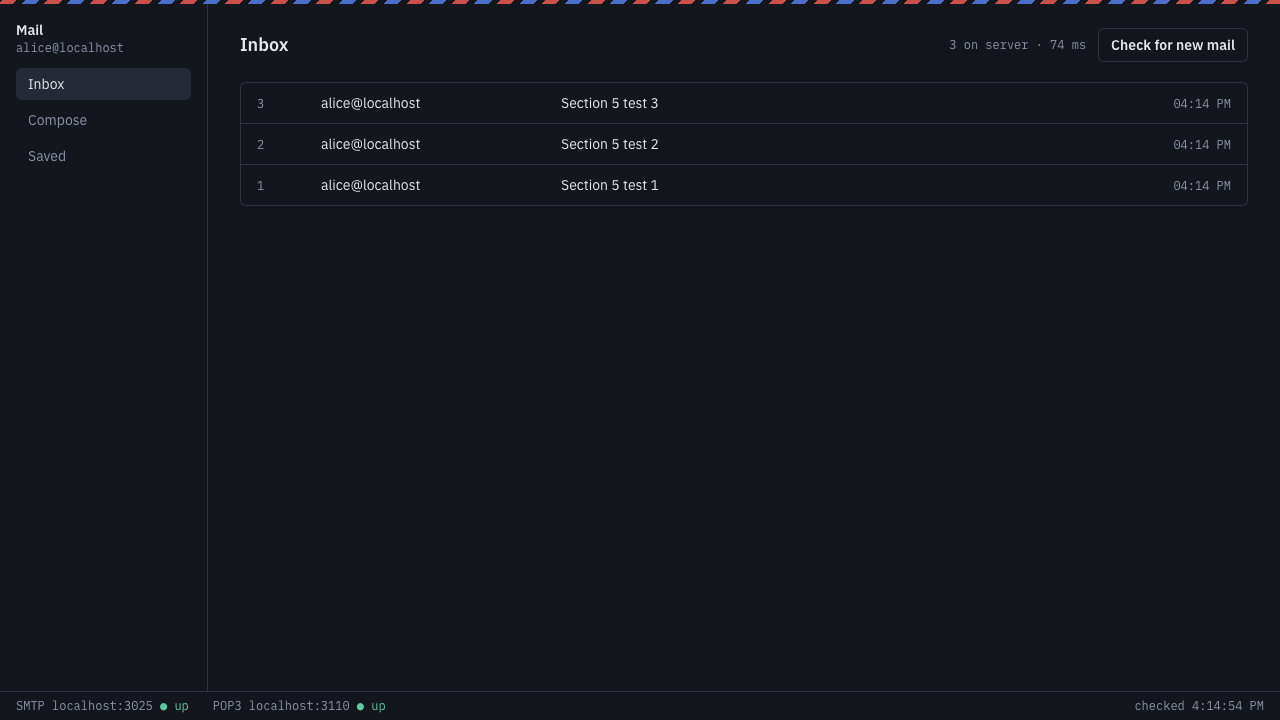
\includegraphics[width=\linewidth]{web-01-inbox.png}\caption{Inbox}\end{subfigure}\hfill
\begin{subfigure}{0.49\linewidth}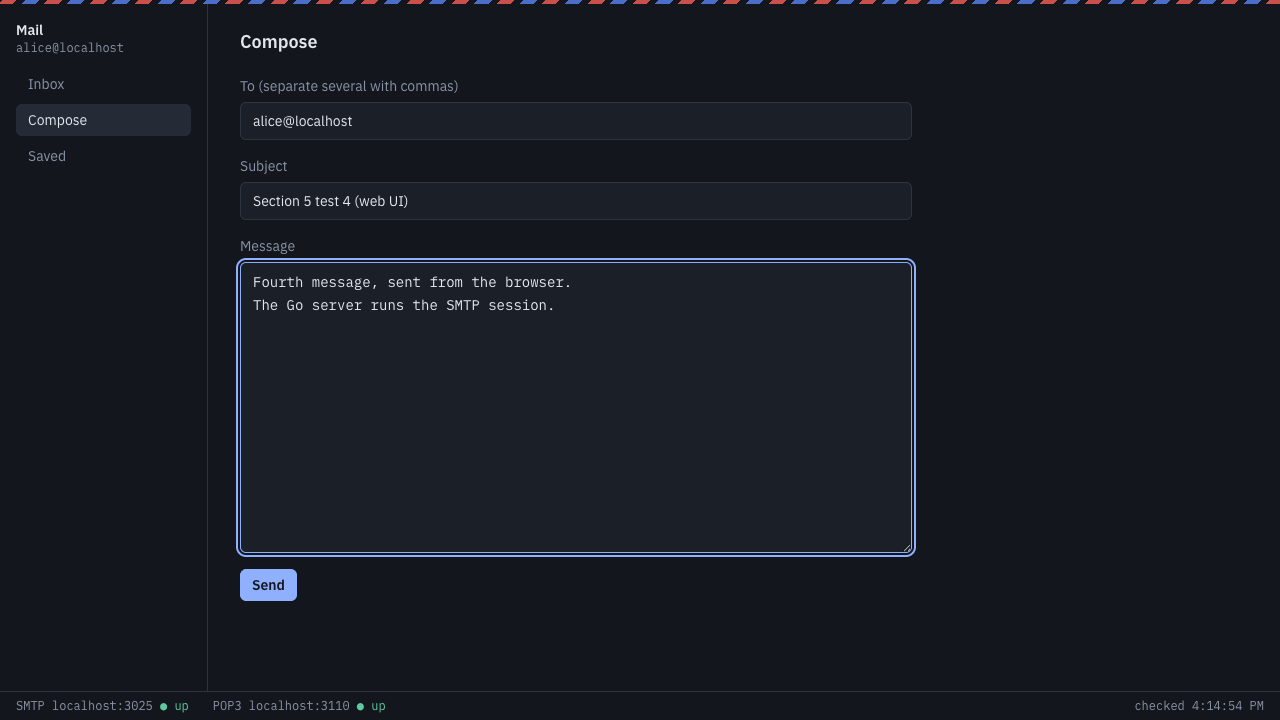
\includegraphics[width=\linewidth]{web-03-compose.png}\caption{Compose}\end{subfigure}\\[0.6em]
\begin{subfigure}{0.49\linewidth}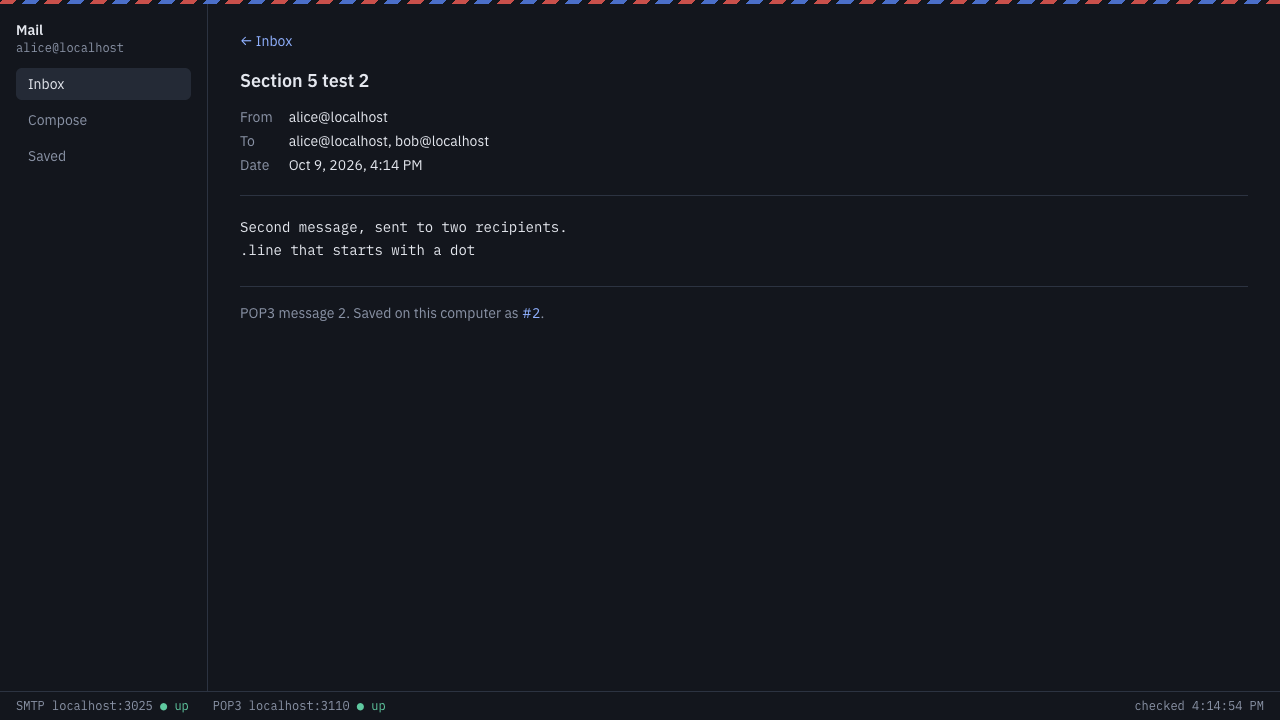
\includegraphics[width=\linewidth]{web-02-read-message.png}\caption{Read message}\end{subfigure}\hfill
\begin{subfigure}{0.49\linewidth}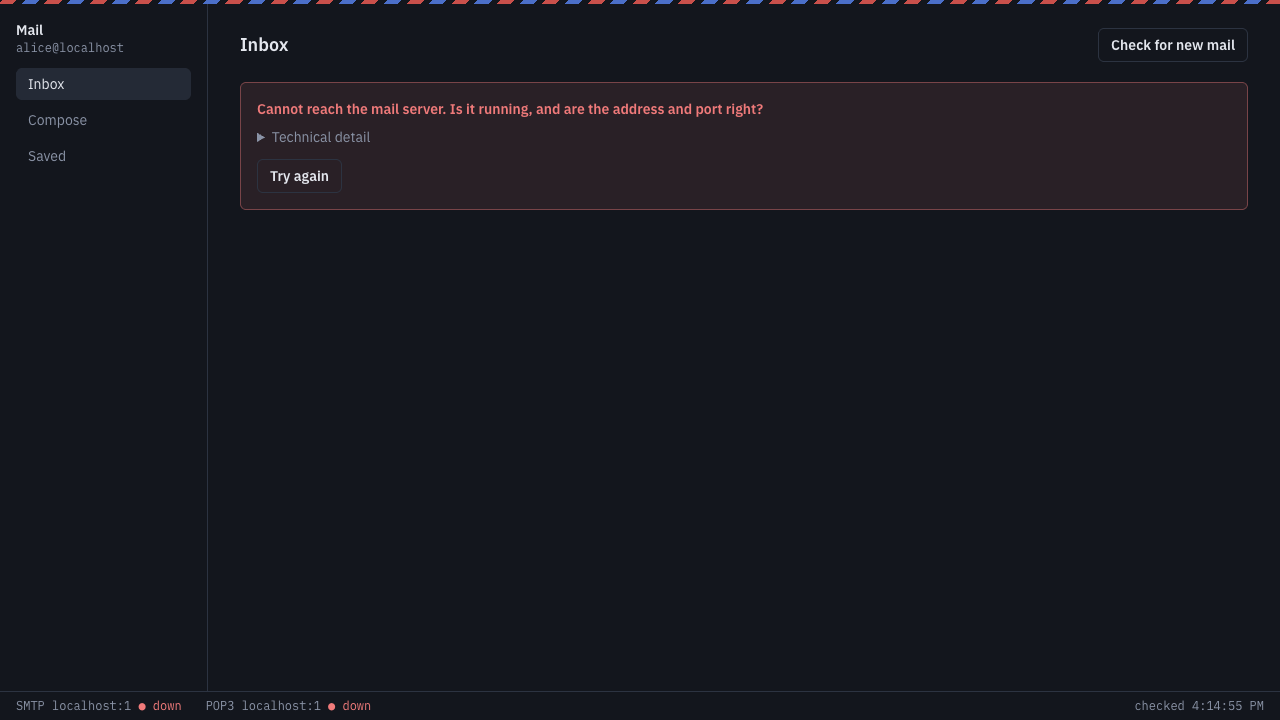
\includegraphics[width=\linewidth]{web-09-error-server-down.png}\caption{Error: server down}\end{subfigure}
\caption{The web interface running the same tests (all screenshots are in
         \texttt{Results/screenshots/}).}
\end{figure}

% =================================================
\section{Performance}
\label{sec:perf}
% =================================================

\texttt{Tests/perf} measures whole protocol sessions (TCP connect, commands, \texttt{QUIT})
against GreenMail on the same machine. Sends and single retrievals ran 10 times per size;
the full inbox check ran 5 times. The bodies are realistic 72-character text lines. The test
uses bob's account so the demo inbox is not filled.

\begin{table}[H]
\centering\small
\caption{Session times in milliseconds (macOS, Apple Silicon, Go 1.26.7, GreenMail 2.1.14 in
         Docker, localhost).}
\label{tab:timing}
\begin{tabular}{@{} l l r r r r @{}}
\toprule
\textbf{Operation} & \textbf{Size} & \textbf{Min} & \textbf{Median} & \textbf{Mean} & \textbf{Max} \\
\midrule
\icon{i-send} Send (SMTP session)       & 1 KB   & 4.9  & 7.8  & 11.9 & 28.3 \\
                                        & 10 KB  & 5.8  & 7.3  & 8.2  & 18.9 \\
                                        & 100 KB & 18.2 & 21.4 & 21.1 & 28.2 \\
\midrule
\icon{i-download} Retrieve one (RETR)   & 1 KB   & 2.6  & 3.0  & 3.1  & 4.1 \\
                                        & 10 KB  & 8.2  & 8.7  & 8.8  & 10.6 \\
                                        & 100 KB & 63.7 & 66.1 & 66.1 & 68.3 \\
\midrule
\icon{i-inbox} Check inbox (LIST + RETR all 31) & mixed & 721.5 & 734.8 & 748.5 & 808.0 \\
\bottomrule
\end{tabular}
\end{table}

\begin{figure}[H]
\centering
\begin{tikzpicture}
\begin{axis}[
  ybar, bar width=14pt, width=0.72\linewidth, height=5.4cm,
  symbolic x coords={1 KB,10 KB,100 KB}, xtick=data,
  ylabel={median time (ms)}, ymin=0, ymax=78,
  nodes near coords, nodes near coords style={font=\scriptsize},
  every node near coord/.append style={/pgf/number format/fixed, /pgf/number format/fixed zerofill, /pgf/number format/precision=1},
  legend style={at={(0.03,0.97)}, anchor=north west, font=\small, draw=rule},
  axis line style={draw=rule}, tick style={draw=rule},
  ymajorgrids, grid style={draw=rule!60},
  enlarge x limits=0.25, tick label style={font=\small}, label style={font=\small},
]
\addplot[fill=accent!75, draw=accent] coordinates {(1 KB,7.8) (10 KB,7.3) (100 KB,21.4)};
\addplot[fill=okc!65, draw=okc] coordinates {(1 KB,3.0) (10 KB,8.7) (100 KB,66.1)};
\legend{Send (SMTP), Retrieve one (POP3)}
\end{axis}
\end{tikzpicture}
\caption{Median send and retrieve times by message size.}
\end{figure}

\textbf{Discussion.}
\begin{itemize}
  \item \textbf{Small messages cost the same.} Sending 1\,KB and 10\,KB both take about
        7--8\,ms. That time is the TCP connect plus five command round trips, not the data.
  \item \textbf{The first session is slower.} The first send in the CLI run took 53\,ms and the
        slowest timed send 28\,ms, against 5--11\,ms for later ones: the first connection
        warms up GreenMail's Java code and Docker's port forwarding. The median ignores this
        outlier, the mean does not, which is why the 1\,KB mean is well above its median.
  \item \textbf{Retrieving 100\,KB takes about three times as long as sending it.} The cause is
        on the server side. A raw Python socket, with no Go code involved, received a
        104\,KB \texttt{RETR} reply in 672 \texttt{recv()} calls of about 155 bytes:
        GreenMail writes roughly one line per TCP segment, and every segment crosses Docker's
        port forwarding. Sending is faster because the client's buffered writer sends large
        segments. The client reassembled all 672 pieces correctly, which is the
        byte-stream property of Section~2.3 in practice.
  \item \textbf{Check Inbox grows with the mailbox.} 31 messages (10 of them 100\,KB) take
        about 0.73\,s, because the client retrieves every message to show its sender, subject
        and date. POP3 \texttt{TOP n 0} (headers only) would make this much cheaper; it is
        not in the required command set and was not implemented.
\end{itemize}

% =================================================
\section{Summary or Conclusions}
% =================================================

\textbf{Completed.} All basic requirements are implemented and tested: configuration with
clear startup errors, SMTP sending to one or more recipients, POP3 receiving with an Inbox and
message view, a local JSON mailbox that survives restarts, handling of every failure kind the
spec lists, and an event log that never contains a password. As bonus features there is a web
interface, sign-in with multiple accounts each with its own mailbox, and concurrency-safe
shared state verified by the race detector. The five required tests pass, as do 51 automated
tests.

\textbf{Main technical problems and their solutions.}
\begin{itemize}
  \item \emph{Multi-line SMTP replies.} GreenMail answers \texttt{EHLO} with three lines.
        Reading only one line per command would match every later reply to the wrong
        command. The client reads the complete reply (all \texttt{250-} continuation lines)
        before sending the next command.
  \item \emph{Partial reads.} A reply can arrive in hundreds of pieces (672 for one 100\,KB
        message). All reads go through a buffered line reader, and completeness is decided
        by the protocol's own end markers, never by the size of a read.
  \item \emph{The end-of-data dot.} A body line holding only ``\texttt{.}'' would end a
        message early. Dot-stuffing is applied on send and removed on receive, and the test
        run includes a body line that starts with a dot.
  \item \emph{POP3 numbers change between sessions.} Saved messages get their own permanent
        ID, and a SHA-256 hash stops the same message being saved twice.
  \item \emph{Passwords in logs.} The \texttt{PASS} line is masked at the protocol layer and
        the logger redacts password attributes; a test checks the log file.
  \item \emph{A server that stops answering.} A blocking read would wait forever. A deadline
        is set before every step, so the client gives up after \texttt{timeout\_seconds}.
  \item \emph{Parallel POP3 logins.} The server locks the maildrop during a session, so two
        browser tabs refreshing at once would collide. POP3 sessions for one account are
        serialised by a mutex.
\end{itemize}

% TODO (student): write this paragraph in your own words.
\textbf{What I learned.} \prompt{Your own reflection: e.g.\ what was harder than expected,
what reading the RFCs taught you (QUIT is answered with 221, not 250), and what testing
against an independent server showed.}

\textbf{Limitations and future work.}
\begin{itemize}
  \item No TLS/STARTTLS and no SMTP AUTH; the client is meant for a local test server.
  \item Check Inbox downloads every message. \texttt{TOP} or \texttt{UIDL} would let it fetch
        headers only, or only new messages.
  \item Messages are never deleted from the server (\texttt{DELE} is not used).
  \item Plain text only: no attachments or HTML mail.
  \item The web session cookie travels over plain HTTP, so the server listens on localhost
        only.
\end{itemize}

% =================================================
\section{References}
% =================================================

\renewcommand{\refname}{}
\vspace{-2.5em}
\begin{thebibliography}{9}
\bibitem{rfc5321} J.~Klensin, ``Simple Mail Transfer Protocol,'' RFC 5321, IETF, Oct.\ 2008. \url{https://www.rfc-editor.org/rfc/rfc5321}
\bibitem{rfc1939} J.~Myers and M.~Rose, ``Post Office Protocol -- Version 3,'' RFC 1939, IETF, May 1996. \url{https://www.rfc-editor.org/rfc/rfc1939}
\bibitem{rfc5322} P.~Resnick, ``Internet Message Format,'' RFC 5322, IETF, Oct.\ 2008. \url{https://www.rfc-editor.org/rfc/rfc5322}
\bibitem{rfc2047} K.~Moore, ``MIME Part Three: Message Header Extensions for Non-ASCII Text,'' RFC 2047, IETF, Nov.\ 1996. \url{https://www.rfc-editor.org/rfc/rfc2047}
\bibitem{gostd} The Go Authors, Go standard library documentation: \texttt{net}, \texttt{net/textproto}, \texttt{net/mail}, \texttt{mime}, \texttt{log/slog}, \texttt{encoding/json}, \texttt{net/http}. \url{https://pkg.go.dev/std}
\bibitem{greenmail} GreenMail, ``GreenMail -- Test suite for email,'' version 2.1.14. \url{https://greenmail-mail-test.github.io/greenmail/}
\bibitem{vite} Vite, ``Vite documentation.'' \url{https://vite.dev}
\bibitem{tailwind} Tailwind Labs, ``Tailwind CSS documentation,'' v4. \url{https://tailwindcss.com/docs}
\bibitem{course} Z.~Liu, ``Design and Implementation of a Lightweight Email Client,'' project description, Computer Network Course Practice, Beijing Institute of Technology, 2026.
\end{thebibliography}

% =================================================
\section{Comments}
% =================================================

% Optional. Write your own comments or suggestions about the course here,
% or delete this section before submission.
\prompt{Optional: comments or suggestions about the course, project, or teaching materials.}

\vfill

\noindent\textbf{Submission note:}
Submit the complete source code, README, this report, representative screenshots/terminal output, test results/logs, and a short description of any bonus features. All work is individual; be prepared to explain the submitted code and protocol behavior during the presentation or demonstration.

\end{document}
